\documentclass[12pt,a4paper,openright,twoside]{report}
\usepackage[italian,english]{babel}
\usepackage{fancyhdr}
\usepackage{indentfirst}
\usepackage{newlfont}
\usepackage{pdfpages}
\usepackage{abstract}
\oddsidemargin=30pt \evensidemargin=20pt
\pagestyle{fancy}\addtolength{\headwidth}{20pt}\setlength{\headheight}{15pt}
\renewcommand{\chaptermark}[1]{\markboth{\thechapter.\ #1}{}}
\renewcommand{\sectionmark}[1]{\markright{\thesection \ #1}{}}
\rhead[\fancyplain{}{\bfseries\leftmark}]{\fancyplain{}{\bfseries\thepage}}
\cfoot{}
\linespread{1.3}
\begin{document}
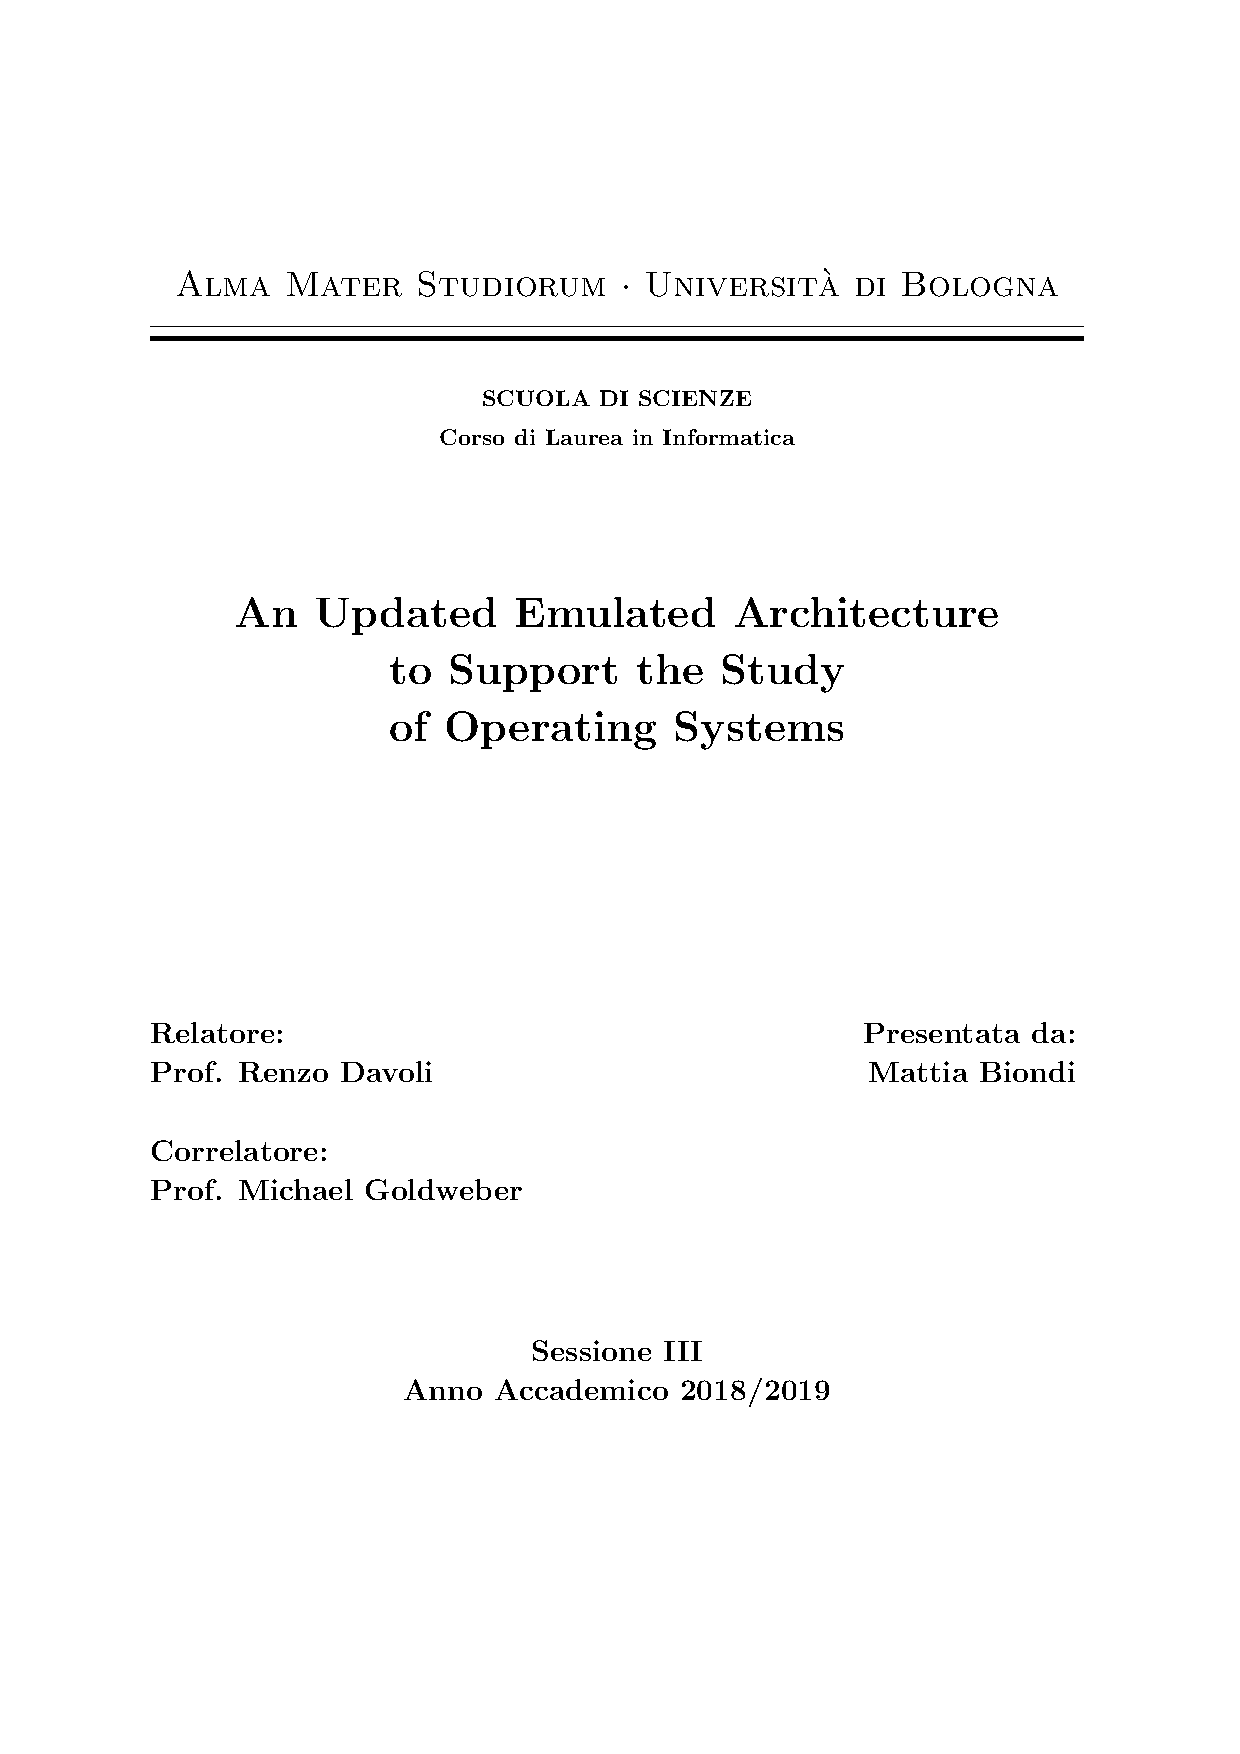
\includepdf[pages=-]{titlepage.pdf}
\clearpage{\pagestyle{empty}\cleardoublepage}
\begin{titlepage}
\thispagestyle{empty}
\topmargin=6.5cm
\raggedleft
\large
\em
Agli amici di sempre,\linebreak
alla mia famiglia,\linebreak
che non mi ha mai impedito nulla,\linebreak
e a Jas,\linebreak
senza la quale non sarei qui oggi.
\newpage
\clearpage{\pagestyle{empty}\cleardoublepage}
\end{titlepage}
\begin{abstract}
One of the most effective way to learn something new is by actively practicing it, and there is---maybe---no better way to study an Operating Systems course than by building your own OS.
It is also true that the realization of an operating system capable of running on a real hardware machine could be an overly complex and unsuitable task for an undergraduated student.
Nonetheless, it is possibile to use simplified computer system simulators in order to achieve the goal of teaching Computer Science foundations in the university environment, thus allowing students to experience a quite realistic rappresentation of an operating system.
$\mu$MPS \cite{umps} has been created for this purpose, a pedagogically appropriate machine emulator, based aroud the MIPS R2/3000 microprocessor, which features an accessible architecture that includes a rich set of easily programmable devices.
$\mu$MPS has an almost two decades old historical development and the outcome of the following thesis is the third version of the software, dubbed $\mu$MPS3.
This second major revision aims to semplify even more the emulator's complexity in order to lighten the load of work required by the students during the OS design and implementation.
Two of these semplifications are the removal of the virtual memory bit, which allowed address translation to be turned on and off, and the replacement of the tape device with a new flash drive device---certainly something more familiar to the new generation of students.
Other major improvements which concern everything from the project building tools to the front-end were made, enabling the upgrade of $\mu$MPS to a modern reliable educational software.
\end{abstract}
\clearpage{\pagestyle{empty}\cleardoublepage}
\tableofcontents
\addtocontents{toc}{\protect\thispagestyle{empty}}
\thispagestyle{empty}
\clearpage{\pagestyle{empty}\cleardoublepage}
\pagenumbering{arabic}
\chapter{Introduction}
\lhead[\fancyplain{}{\bfseries\thepage}]{\fancyplain{}{\bfseries\rightmark}}
\section{Background}
The study and the design of how an operating system works is a long established practice in every Computer Science's curriculum.
The approach on practical contexts is crucial to fully understand how a machine works behind the theoretical notions studied in the early stages of the course of study, and it is usually followed by the decision of which processor architecture is the best teaching choice.
Obviously, there is not only one approach of how the software can interface with the hardware, and while older implementation---although applicable for educational purposes---are now obsolete and incompatible with current platforms, modern ones are designed with high quality and speed in mind, which makes them overly complex and unsuitable for pedagogic experience.
The MIPS architecture became one of the landmarks in this choice over the years due to its clean and elegant instruction set, despite being excessively convoluted to student’s perception because of the level of details obscuring the basic underlying feature of it.
A potential solution to the problem is the adoption of simplified computer system simulators like $\mu$MPS, in order to bring together an adeguate level of understanding and a realistic rappresentation of an operating system.
\section{History of $\mu$MPS}
\section{$\mu$MPS3}
\section{Document's Structure}
\chapter{Memory Management}
\lhead[\fancyplain{}{\bfseries\thepage}]{\fancyplain{}{\bfseries\rightmark}}

\section{Primary Design}
\section{TLB Floor Address}
\section{VM Bit Removal}
\chapter{Exception Handling}
\lhead[\fancyplain{}{\bfseries\thepage}]{\fancyplain{}{\bfseries\rightmark}}
\section{Primary Design}
\section{BIOS Data area}
\lhead[\fancyplain{}{\bfseries\thepage}]{\fancyplain{}{\bfseries\rightmark}}
\chapter{Flash Devices}
\lhead[\fancyplain{}{\bfseries\thepage}]{\fancyplain{}{\bfseries\rightmark}}
\section{Tape Readers}
\section{Flash Drives}
\chapter{Project Modernization}
\lhead[\fancyplain{}{\bfseries\thepage}]{\fancyplain{}{\bfseries\rightmark}}
\section{CMake Migration}
\section{Qt5 Transition}
\section{Logo and Icon Theme}
\chapter{Linux Packaging}
\lhead[\fancyplain{}{\bfseries\thepage}]{\fancyplain{}{\bfseries\rightmark}}
\section{Debian Package}
\section{Arch Linux Package}
\chapter{Conclusions}
\lhead[\fancyplain{}{\bfseries\thepage}]{\fancyplain{}{\bfseries\rightmark}}
Knowing how an operating system works should be common knowledge and not something restricted  only to the ones who studied in the IT field.
If you are reading this document there are high chances you are doing it on a device of your property, which is running an operating system, and you should know how all of this really works in other to really feel like you own this particular system.
\begin{thebibliography}{99}
\addcontentsline{toc}{chapter}{Bibliography}
\bibitem{umps}
  M. Goldweber, R. Davoli, and M. Morsiani,
  \textit{The Kaya OS project and the $\mu$MPS hardware emulator},
   SIGCSE Bull.,
   vol. 37, pp. 49–53,
   June 2005.
\end{thebibliography}
\end{document}
